\chapter{Performance}
 \label{chap:perf}
 
 The major goal of this work is to have a fully automated model generation in PyNEST without drastically degrading the performance of the simulation script and encouraging users to use the new implemented JIT module. In order to test the impact of the using the JIT module in the simulation script, we need to test different configurations that might eventually appear when running the simulation with JIT. Firstly, we test the neuronal network with a custom neuron and built-in synapse model with the script explicitly calling PyNESTML module and the \texttt{nest.Install} function and  consider its running time as our baseline. Secondly, we run the same neuronal network, but this time everything is controlled by the JIT module. Thirdly, we repeat the same experiment, but this time we choose a neuronal network that includes a custom implemented synapse model.
 
 As the NestKernel does not completely utilize the new data structure behind vectorization, we can not really make meaningful evaluation of its impact on the performance. Therefore, we only decided to compare single functions between simple and vectorized models. Such functions are \texttt{nest.Create} and \texttt{nest.GetStatus}.
 
 From the JIT tool perspective, we do not really care about the size of the network or its behavior, because we only simply retrieve the model and make it available to the simulation script. In that case, any neuronal network should be fine to test with. In the first experiment, we choose a random balanced network as  described by \citet{brunel2000dynamics}. For the second experiment with a custom synapse model, we build a network with a spike-timing dependent plasticity (STDP) synapse.
 
 
 For vectorization, we only test the \texttt{nest.Create} and \texttt{nest.GetStatus} functions by creating instances of the \emph{Izhikevich} \citep{1257420} neuron model with modifying the number of instances of the model and the number of used threads.
 
\section{The JIT Module}

\subsection{Running The JIT Module Without An external Synapse Type}

In the first experiment in testing the JIT module, we run the \emph{Brunel} network by explicitly using PyNESTML to generate the code for the required model, and then we run the same network by using the JIT module. The result of the experiment can be found in the \autoref{fig:max_average_min}.

\begin{figure}[ht!]
    \centering
    \includegraphics[width=\textwidth]{src/pic/box_plot_three.png}
    \caption{\textbf{Network with custom neuron and built-in synapse}: The blue box represents the performance of the simulation script without using JIT, and it has the best performance among the other experiments. The orange box represents the performance of running the same neural network with JIT, but with the model being an external model in a dynamic library. Finally, the green box shows the runtime of the simulation with JIT, with the neuron model only available in a NESTML file format. The red lines inside each box represent the average runtime of the experiments.}
    \label{fig:max_average_min}
\end{figure}

In the \autoref{fig:max_average_min}, we show the box plot for three different possible cases that might appear when running the simulation script. The first box (the blue box) represents the runtime when running the simulation script with explicitly calling the PyNESTML module and manually generating the code for the neuron model. The second box (the orange box) represents the runtime when running the simulation with the JIT module with the neuron model being already built in the library. Lastly, the green box represents the runtime when running the simulation with the JIT module and with the neuron model being solely in a NESTML format. All the three experiments share the same network topology and only differ in the way how the model instances are loaded and created. We run each experiment 20 times, and in each run we store the runtime of the whole simulation script.

The first case (i.e., \emph{Without\_Jit}) has the lowest runtime, and it took on average 90 seconds to finish the simulation. On the other hand, the average runtime for the \emph{Jit\_Lib} took around 90 seconds, and the \emph{Jit\_Nestml} took around 120 seconds.  Both the first case and the second case have almost the same behavior, with the exception that the \emph{minimum} runtime for the second case was around 3 seconds slower. This can be explained with the introduced overhead in the JIT module, and it is the most significant in the last case. All the three values of the \emph{Jit\_Nestml} are the highest among the other cases, and it can be explained by the time required for searching the model and maintaining \texttt{NodeCollectionProxy} by converting the \texttt{JitNodeCollection} to the real \texttt{NodeCollection} instances and copying the parameters from one instance to the other.


\subsection*{Running The JIT Module with An external Synapse Type}

In the second experiment, we ran the \emph{STDP windows} simulation script from the NESTML tutorial which uses a custom STDP synapse model, and again we compared the simulation runtime using the JIT module against the original script. In this tutorial, we have a function that is responsible for creating the instances of the models and creating the network, and it is called multiple times in a \emph{for-loop} (exactly 151 times). In the JIT tool settings, it means that the model will be searched many times, and we would expect that only the first iteration will take most of the time in comparison to the subsequent iterations. 

\begin{figure}[ht!]
    \centering
    \includegraphics[width=\textwidth]{src/pic/three_plots.png}
    \caption{\textbf{Network with custom neuron and built-in synapse}: The first plot \emph{a} represents the overall runtime of the three experiments. The second plot \emph{b} shows the average runtime of the first iteration in all of the three experiments. In the last plot \emph{c}, we compute the average runtime for all iterations for each run and then take the average runtime over multiple runs.}
    \label{fig:overall_runtime}
\end{figure}

In \autoref{fig:overall_runtime}, we analyze the runtime of the whole script, and then we take a look at the runtime of the function responsible for creating the network in each iteration. At the top left in the figure, plot \emph{a}, we can observe the significant effect of using the JIT module with an external synapse type. The JIT module requires on average around 650 seconds, whereas the normal execution took around 50 seconds to finish. The minimum runtime of the JIT approach is also very high in comparison to the normal mode. If we observe the second plot, plot \emph{b}, at the top, we can straightforward see the reason behind the 700 seconds runtime. The first iteration alone took more than 40 seconds to finish, whereas the normal execution took less than one second to finish. This difference is caused by the same overhead discussed above, plus now we have to trigger the code generation pipeline again and replace the \emph{source/target} elements in the network with the new correct neuron model and update its state with the synapse instance. 

In the third plot, plot \emph{c}, at the bottom left of the figure, we show the average time needed by all the 151 iterations in each run. The most left box representing the baseline of the experiment is almost the same as the one in the plot \emph{b}, which means that all runs of the function take on average the same amount of time. However, the other two experiments show a slight change in the runtime. The average runtime for both experiments using the JIT module have lower values than the box on the top right plot \emph{b}. The reason behind it is that the first iteration requires more time to find the model and make it available, whereas the subsequent iterations are only affected by the overhead of maintaining the logic of the JIT mechanism in the background.



\section{Vectoriztation}

As NestKernel does not completely support vectorization yet, we restrict our tests to the direct functions involved with the vectorized model. We tested both the \texttt{nest.Create} and \texttt{nest.GetStatus} functions. Both experiments share the same configuration, mainly, we can either change the number of created nodes and keep the number of threads constant or vice-versa. The experiments are executed on a \emph{Ryzen 7 3700u} processor with four cores and eight threads.

For the number of the nodes, we have picked \{1, 10, 30, 50, 100, 300, 500, 2000, 5000, 8000, 1000\} and for the number of threads we have \{1, 2, 4, 8, 16, 32\}. Each sub-experiment is run five times, by storing the \emph{Wall} time as the real elasped time of executing the single functions in a \emph{csv} file containing the runtime of the \emph{vectorized} and \emph{non-vectorized} model. In each sub-experiment, we have three plots. In the first plot on the left, we show the \emph{max-average-min} runtime of the \emph{vectorized} model. The middle plot shows the \emph{max-average-min} runtime of the simple \emph{non-vectorized} model. Finally, the last plot on the right, overlays the average runtime for both models in a single plot. The \emph{y-axis} in the first two plots shows the values after applying the \emph{logarithmic} function with base 10 on the runtime values, which are stored in microseconds, whereas the values in the last plot are only in microseconds.

\subsection{The \texttt{Create} function}

\subsubsection{Varying the number of nodes with a constant number of threads}

 In the first configuration in testing the \texttt{nest.Create} function, we fix the number of threads and vary the number of nodes. From the  \autoref{fig:threads_1} until \autoref{fig:threads_32}, we show the results of the experiments. For each number of threads, we display the performance of the \texttt{nest.Create} function with the vectorized model against the non-vectorized models. 


In \autoref{fig:threads_1}, we observe that both types of models behave the same until reaching a number of nodes larger than 300 ($10^{2.5}$). The gap between the two models might be explained by the overhead required to resize the container of the vectorized model, as an reallocation of the data might take place when increasing the size of the container. After that point, the vectorized model starts to become a bit slower on average, but by a few microseconds. Another observation is that the min-max area of the vectorized model is a bit wide and gets more narrow after reaching $10^3$, whereas the min-max area for the non-vectorized model is almost always narrow, and it gets more narrow after reaching 300 nodes.

In \autoref{fig:threads_2}, we observe the same performance for both types of models, even the \emph{max-min} area looks almost the same. As in the previous experience, the performance of the vectorized model becomes a bit slower after reaching 300 nodes with a few milliseconds in comparison to the non-vectorized model. In \autoref{fig:threads_4} with four threads, we have the same observation as in the \autoref{fig:threads_2} with two threads.

In the rest of the figures with threads in \{8, 16, 32\}, we observe that the vectorized model gets slower and the gap between both models gets wider but still in the range of a few milliseconds.

\begin{figure}[t!]
    \centering
    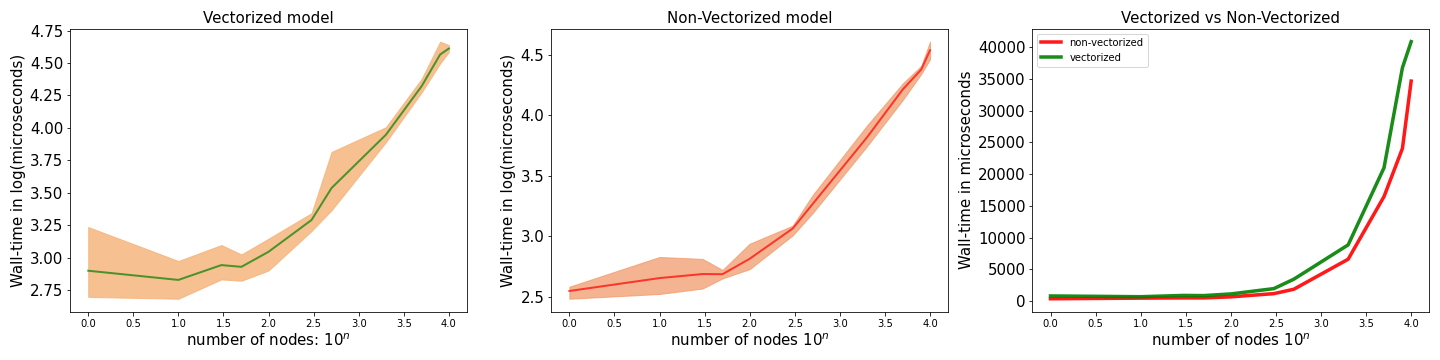
\includegraphics[width=\textwidth]{src/pic/thread_1.png}
    \caption{\textbf{Performance of \texttt{nest.Create} function with the number of threads=1}: The left plot depicts the average performance of the vectorized model. The plot in the model shows the average performance of the original non-vectorized model in NEST. The last plot in the right overlays the average performance of both models. Additionally, in the first two plots in the left, we show the min-max area, and it is depicted in orange and red respectively.}
    \label{fig:threads_1}
\end{figure}
\begin{figure}[t!]
    \centering
    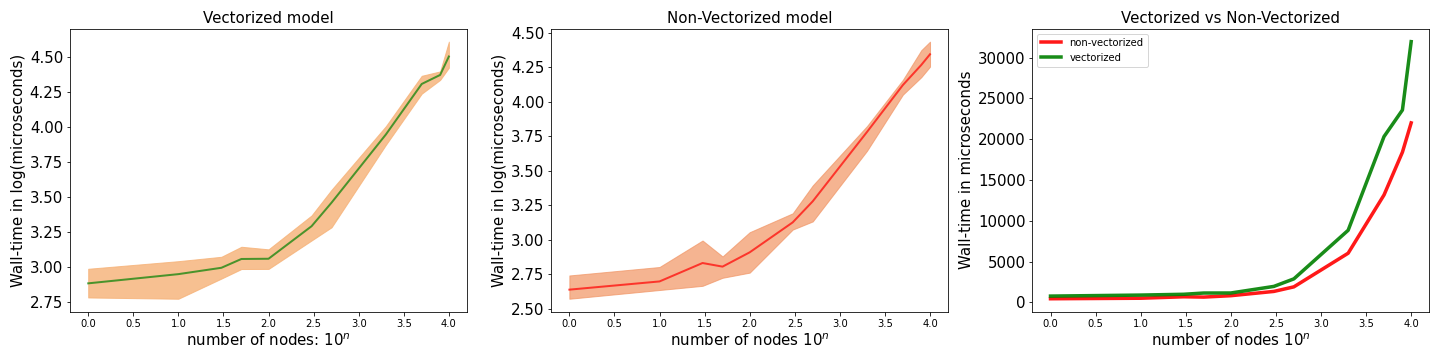
\includegraphics[width=\textwidth]{src/pic/thread_2.png}
    \caption{\textbf{Performance of \texttt{nest.Create} function with the number of threads=2}: For description see \autoref{fig:threads_1}.}
    \label{fig:threads_2}
\end{figure}

\begin{figure}[t!]
    \centering
    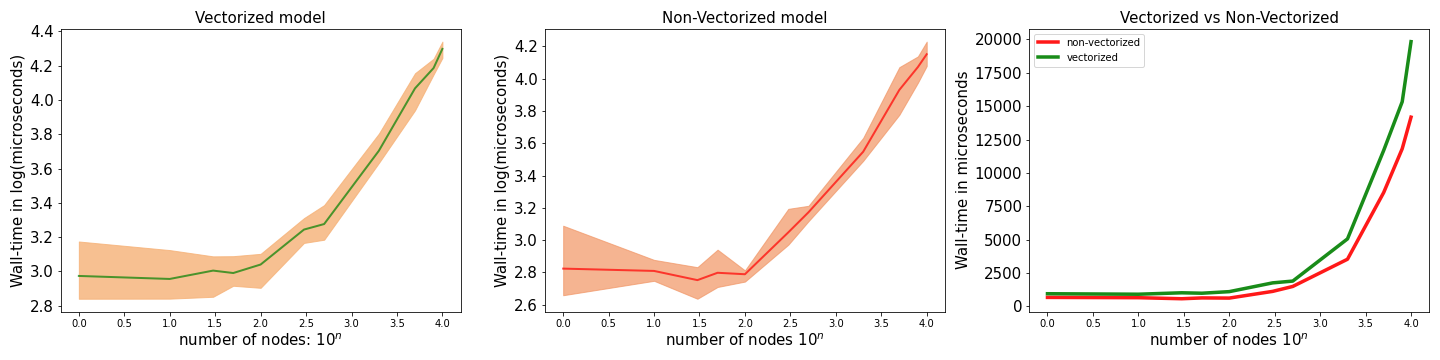
\includegraphics[width=\textwidth]{src/pic/thread_4.png}
    \caption{\textbf{Performance of \texttt{nest.Create} function with the number of threads=4}: For description see \autoref{fig:threads_1}.}
    \label{fig:threads_4}
\end{figure}

\begin{figure}[t!]
    \centering
    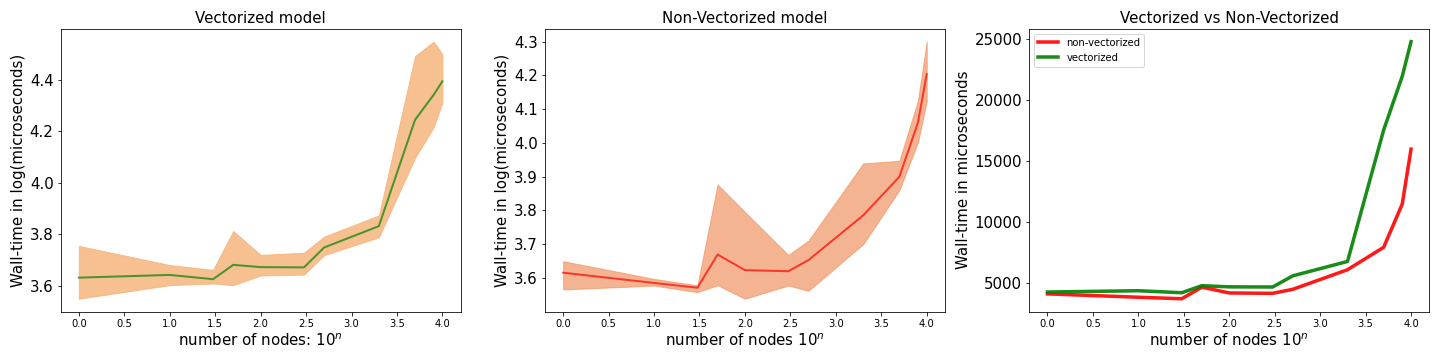
\includegraphics[width=\textwidth]{src/pic/thread_8.png}
    \caption{\textbf{Performance of \texttt{nest.Create} function with the number of threads=8}: For description see \autoref{fig:threads_1}.}
    \label{fig:threads_8}
\end{figure}


\begin{figure}[t!]
    \centering
    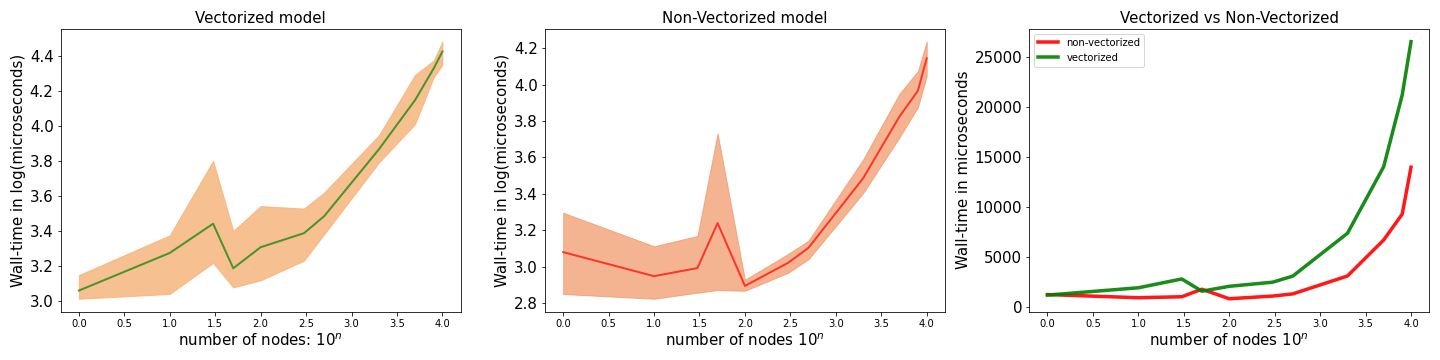
\includegraphics[width=\textwidth]{src/pic/thread_16.png}
    \caption{\textbf{Performance of \texttt{nest.Create} function with the number of threads=16}: For description see \autoref{fig:threads_1}.}
    \label{fig:threads_16}
\end{figure}

\begin{figure}[t!]
    \centering
    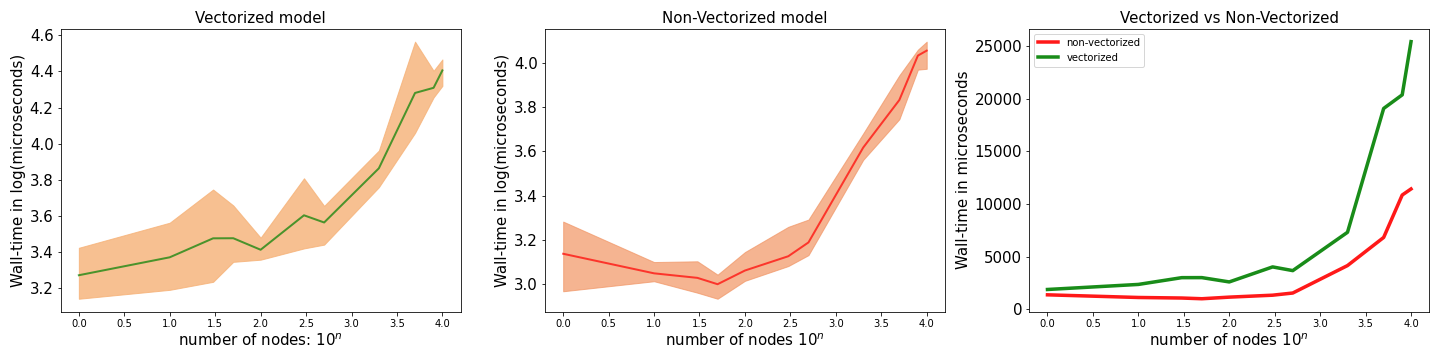
\includegraphics[width=\textwidth]{src/pic/thread_32.png}
    \caption{\textbf{Performance of \texttt{nest.Create} function with the number of threads=32}: For description see \autoref{fig:threads_1}.}
    \label{fig:threads_32}
\end{figure}

\subsubsection{Varying the number of threads with a constant number of nodes}


In general, the plots between \autoref{fig:nodes_1} and \autoref{fig:nodes_10000} show that the \texttt{nest.Create} function has a consistent behavior. In all the plots, we can observe the discontinuity that happens around the points where the number of threads are 4, 8 and 16. At these points the slope changes significantly, and the reason behind it is the processor specification. Recall that we ran the experiments on a four-core processor. In general, the vectorized model is a bit slower than the non-vectorized model and the largest difference can be observed in the \autoref{fig:nodes_5000} with 5000 nodes. In the worst case the vectorized model took around 0.02 seconds creating 5000 nodes with 32 threads, wheras the non-vectorized model took around 0.006 seconds. The difference can be explained by the overhead coming from the virtual functions and the resize function that must allocate enough space for the 5000 nodes.

\foreach \n in {1, 10, 30, 50, 100, 300, 500, 2000, 5000, 8000, 10000}
{
\begin{figure}[t!]
    \centering
    \includegraphics[width=\textwidth]{src/pic/nodes_\n.png}
    \caption{\textbf{Performance of \texttt{nest.Create} function with the number of nodes=\n}: For description see \autoref{fig:threads_1}.}
    \label{fig:nodes_\n}
\end{figure}
}

\subsubsection{The GetStatus function}

\subsubsection*{Varying the number of nodes with a constant number of threads}

Even with the \texttt{nest.GetStatus} not fully being optimized to support vectorization, both the vectorized model and the non-vectorized one has the same performance, with the vectorized model being slightly better with a few microseconds.

\foreach \n in {2, 4, 8, 16, 32}
{
\begin{figure}[t!]
    \centering
    \includegraphics[width=\textwidth]{src/pic/get_thread_\n.png}
    \caption{\textbf{Performance of \texttt{nest.GetStatus} function with the number of nodes=\n}: For description see \autoref{fig:threads_1}.}
    \label{fig:get_threads_\n}
\end{figure}
}

\subsubsection*{Varying the number of threads with a constant number of nodes}

The \texttt{nest.GetStatus} with varying the number of threads has a very different behavior. In \autoref{fig:get_nodes_1}, both models have the same direction of variation with the only difference that at $threads=16$ we observe that the vectorized model is becoming a bit faster. The min-max area in both models is also almost the same. With the number of nodes equal to 10 in \autoref{fig:get_nodes_10}, we observe that between the points with number of threads equal to 6 and 16 the vectorized model is significantly faster, but then starting from 16 the vectorized model becomes slower again.


In \autoref{fig:get_nodes_30}, both  models have the same behavior, with the vectorized model being a bit faster between the points 3 and 14 and then again after 20. Both min-max areas have almost the same shape. In \autoref{fig:get_nodes_50}, the average performance between the models is significantly slower with 1500 microseconds on average. Again, we directly observe the points where the slope of the curves changes. Those points are at position 4, 8 and 16. \autoref{fig:get_nodes_30} with 100 nodes shows also the same observations as in the \autoref{fig:get_nodes_30}.

In \autoref{fig:get_nodes_300} with 300 nodes, the vectorized model takes almost completely the lead in all thread values, with the only exception between position 6 and 10. Both \autoref{fig:get_nodes_500} and \autoref{fig:get_nodes_2000} respectively with 500 and 2000 nodes show the same observations, where the vectorized model is being faster than the simple model.

Reaching higher number of nodes as in \autoref{fig:get_nodes_8000} with 8000 nodes and in \autoref{fig:get_nodes_10000} with 10000 nodes, the vectorized model is either behaving the same as the simple model or performing even better. This might be the cause of the overhead required of the non-vectorized model to constantly keep calling the constructor over and over, whereas in the vectorized model we only call it once, but also we still have the overhead of the resize function call. In general, with the current state of the vectorized model we might conclude that with number of nodes larger than 1000, the vectorized will behave better.



\foreach \n in {1, 10, 30, 50, 100, 300, 500, 2000, 5000, 8000, 10000}
{
\begin{figure}[t!]
    \includegraphics[width=\textwidth]{src/pic/get_nodes_\n.png}
    \caption{\textbf{Performance of \texttt{nest.GetStatus} function with the number of threads=\n}: For description see \autoref{fig:threads_1}.}
    \label{fig:get_nodes_\n}
\end{figure}
}




With the current implementation, the vectorization in its first prototype shows promissing results. The difference between the vectorized model and the non-vectorized is within fraction of seconds, and does not drastically impact NEST's performance. The next steps will be having a complete integration of the vectroization in the NestKernel and not only adjust the \texttt{GetStatus} function, but also the internal functions in NEST as the \texttt{update} function. The JIT module should then be combined with the vectorization to componsate for the slower behavior when using custom neuron and synapse models toghether in the connect calls.


\afterpage{\blankpage}
\cleardoublepage
